% Copyright Luke Olson 2009--2014
% This work is licensed under the Creative Commons
% Attribution-NonCommercial-NoDerivatives 4.0 International License. To view a
% copy of this license, visit http://creativecommons.org/licenses/by-nc-nd/4.0/.
%
\documentclass[10pt]{beamer}
%\documentclass[handout,10pt]{beamer}
%pdflatex -jobname lecture15.print lecture15
%
\mode<presentation>
{
  \usetheme[secheader]{Boadilla}
  \usefonttheme[onlymath]{serif}
  \setbeamercovered{invisible}
  \usecolortheme{luke}
  %\setbeamercovered{transparent}
  %
}
\mode<handout>
{
  \usetheme[secheader]{Boadilla}
  \usefonttheme[onlymath]{serif}
  \setbeamercovered{invisible}
  \usecolortheme{luke2}
  %\setbeamercovered{transparent}
}
\usepackage{pgf,pgfarrows,pgfnodes,pgfautomata,pgfheaps,pgfshade}
\usepackage{pxfonts}
\usepackage{eulervm}
\usepackage{listings}
\usepackage{url}
%\usepackage{pgfpages}
%\pgfpagesuselayout{2 on 1}[letterpaper]
%
%
%%%%%%%%%%%%%%%%%%%%%%%%%%%%%%%%%%%%%%%%%%%%%%%%%%%%%%%%%%%%%%%%%%%%%%%%


%
%
%
\newcommand{\vb}{{\bf{b}}}
\newcommand{\ve}{{\bf{e}}}
\newcommand{\vg}{{\bf{g}}}
\newcommand{\vp}{{\bf{p}}}
\newcommand{\vr}{{\bf{r}}}
\newcommand{\vu}{{\bf{u}}}
\newcommand{\vx}{{\bf{x}}}
\newcommand{\vz}{{\bf{z}}}
\newcommand{\vA}{{\bf{A}}}
\newcommand{\vP}{{\bf{P}}}
\newcommand{\vU}{{\bf{U}}}
\newcommand{\mO}{{\mathcal{O}}}
\newcommand{\mF}{{\mathcal{F}}}
\definecolor{mygray}{rgb}{0.95,0.95,0.95}
\lstset{
        language=matlab,
        numbers=left, numberstyle=\tiny, stepnumber=1, numbersep=5pt,
        basicstyle=\color{black}\ttfamily\small,
        commentstyle=\color{green}\ttfamily,
        keywordstyle=\color{blue}\ttfamily,
        stringstyle=\color{red}\ttfamily,
        showstringspaces=false,
        backgroundcolor=\color{mygray},
        breaklines,
}
\newcommand{\norm}[1]{{\ensuremath{{\|#1\|}}}}
\newcommand{\matdim}[2]{\ensuremath{#1\times#2}}
\newcommand{\rank}[1]{\ensuremath{\mathrm{rank}(#1)}}
\newcommand{\epsm}{\ensuremath{\varepsilon_m}}
\newcommand{\cmd}[1]{{\normalfont\ttfamily\bfseries#1}}

\author{L. Olson}
\institute[UIUC]
{Department of Computer Science\\
University of Illinois at Urbana-Champaign\\
\vspace{0.5cm}
}
%%%%%%%%%%%%%%%%%%%%%%%%%%%%%%%%%%%%%%%%%%%%%%%%%%%%%%%%%%%%%%%%%%%%%%%%
\pgfdeclareimage[height=0.5cm]{university-logo}{./figs/uiuclogo}
\logo{\pgfuseimage{university-logo}}
%%%%%%%%%%%%%%%%%%%%%%%%%%%%%%%%%%%%%%%%%%%%%%%%%%%%%%%%%%%%%%%%%%%%%%%%
\title[CS 357]{Lecture 16}
\subtitle{Splines and B\'ezier Curves}
\date{October 20, 2009}

\begin{document}
% -------------------------------------------------
\begin{frame}
  \titlepage
\end{frame}
% -------------------------------------------------
%%%%%%%%%%%%%%%%%%%%%%%%%%%%%%%%%%%%%%%%%%%%%%%%%%%%%%%%%%%%%%%%%%%%%%%%
\begin{frame}
\frametitle{degree 1 spline}
\begin{block}{definition}
A function $S(x)$ is a spline of degree 1 if:
\begin{enumerate}
  \item The domain of $S(x)$ is an interval $[a,b]$
  \item $S(x)$ is continuous on $[a,b]$
  \item There is a partition $a=t_0<t_1<\dots<t_n=b$ such that $S(x)$ is
linear on each subinterval $[t_i,t_{i+1}]$.
\end{enumerate}
\end{block}
\begin{columns}
\begin{column}{0.45\textwidth}
\begin{example}
\begin{equation*}
  S(x) = \begin{cases}
  x & x \in [-1,0]\\
  1 & x \in (0,1)\\
  2x-2 & x \in [1,2]\\
\end{cases}
\end{equation*}
\end{example}
\end{column}
\begin{column}{0.45\textwidth}
\begin{center}
  \pgfimage[width=4.5cm]{./figs/spline3}
\end{center}
\end{column}
\end{columns}
\end{frame}
%%%%%%%%%%%%%%%%%%%%%%%%%%%%%%%%%%%%%%%%%%%%%%%%%%%%%%%%%%%%%%%%%%%%%%%%
%%%%%%%%%%%%%%%%%%%%%%%%%%%%%%%%%%%%%%%%%%%%%%%%%%%%%%%%%%%%%%%%%%%%%%%%
\begin{frame}
\frametitle{degree 1 spline}
Given data $t_0,\dots,t_n$ and $y_0,\dots,y_n$, how do we form a spline?

We need two things to hold in the interval $[a,b]=[t_0,t_n]$:
\begin{enumerate}
  \item $S(t_i) = y_i$ for $i=0,\dots,n$
  \item $S_i(x) = a_ix +b_i$ for $i=0,\dots,n$
\end{enumerate}
Write $S_i(x)$ in point-slope form
\begin{align*}
  S_i(x) & = y_i + m_i(x-t_i)\\
         & = y_i + \frac{y_{i+1}-y_i}{t_{i+1}-t_i}(x-t_i)
\end{align*}
Done.
\end{frame}
%%%%%%%%%%%%%%%%%%%%%%%%%%%%%%%%%%%%%%%%%%%%%%%%%%%%%%%%%%%%%%%%%%%%%%%%
%%%%%%%%%%%%%%%%%%%%%%%%%%%%%%%%%%%%%%%%%%%%%%%%%%%%%%%%%%%%%%%%%%%%%%%%
\begin{frame}[fragile]
\frametitle{degree 1 spline}
\begin{lstlisting}[mathescape]
  input $t,y$ vectors of data
  input evaluation location $x$
  find interval $i$ with $x\in[t_i,t_{i+1}]$
  S = y_i + (x-t_i) m_i
\end{lstlisting}
\end{frame}
%%%%%%%%%%%%%%%%%%%%%%%%%%%%%%%%%%%%%%%%%%%%%%%%%%%%%%%%%%%%%%%%%%%%%%%%
%%%%%%%%%%%%%%%%%%%%%%%%%%%%%%%%%%%%%%%%%%%%%%%%%%%%%%%%%%%%%%%%%%%%%%%%
\begin{frame}
\frametitle{degree 1 spline}
Interesting:
\begin{itemize}
  \item input $n+1$ data points $t_0,\dots,t_n$,$y_0,\dots,y_n$
  \item in each interval we have $S_i(x) = a_i x + b_i$
  \item 2 unknowns per interval $[t_i,t_{i+1}]$
  \item or $2n$ total unknowns
  \item the $n+1$ pieces of input contraints $S(t_i)=y_i$ gives 2
constraints per interval
  \item or $2n$ total constraints 
\end{itemize}
\end{frame}
%%%%%%%%%%%%%%%%%%%%%%%%%%%%%%%%%%%%%%%%%%%%%%%%%%%%%%%%%%%%%%%%%%%%%%%%
%%%%%%%%%%%%%%%%%%%%%%%%%%%%%%%%%%%%%%%%%%%%%%%%%%%%%%%%%%%%%%%%%%%%%%%%
\begin{frame}
\frametitle{degree 2 splines}
\begin{block}{definition}
A function $S(x)$ is a spline of degree 2 if:
\begin{enumerate}
  \item The domain of $S(x)$ is an interval $[a,b]$
  \item $S(x)$ is continuous on $[a,b]$
  \item $S'(x)$ is continuous on $[a,b]$
  \item There is a partition $a=t_0<t_1<\dots<t_n=b$ such that $S(x)$ is
quadratic on each subinterval $[t_i,t_{i+1}]$.
\end{enumerate}
\end{block}
\end{frame}
%%%%%%%%%%%%%%%%%%%%%%%%%%%%%%%%%%%%%%%%%%%%%%%%%%%%%%%%%%%%%%%%%%%%%%%%
%%%%%%%%%%%%%%%%%%%%%%%%%%%%%%%%%%%%%%%%%%%%%%%%%%%%%%%%%%%%%%%%%%%%%%%%
\begin{frame}
\frametitle{degree 2 splines}
\begin{equation*}
  S(x) = \begin{cases}
  S_0(x) &  x\in[t_0,t_1]\\
  S_1(x) &  x\in[t_1,t_2]\\
  \vdots & \vdots \\
  S_{n-1}(x) &  x\in[t_{n-1},t_n]\\
\end{cases}
\end{equation*}
for each $i$ we have
\begin{equation*}
  S_i(x) = a_i x^2 + b_i x + c_i
\end{equation*}
What are $a_i$, $b_i$, $c_i$?
\end{frame}
%%%%%%%%%%%%%%%%%%%%%%%%%%%%%%%%%%%%%%%%%%%%%%%%%%%%%%%%%%%%%%%%%%%%%%%%
%%%%%%%%%%%%%%%%%%%%%%%%%%%%%%%%%%%%%%%%%%%%%%%%%%%%%%%%%%%%%%%%%%%%%%%%
\begin{frame}
\frametitle{degree 2 splines}
\begin{itemize}
  \item 3 unknowns in each interval
  \item $3n$ total unknowns
  \item $2n$ constraints for matching up the input data (2 per interval)
  \item $n-1$ interior points require continuity of the derivative:
$S_{i}'(x_{i+1}) = S_{i+1}'(x_{i+1})$
  \item but this is just $n-1$ constraints
  \item total of $3n-1$ constraints
  \item extra constraint: $S'(x_0)=$given, for example.
\end{itemize}
\end{frame}
%%%%%%%%%%%%%%%%%%%%%%%%%%%%%%%%%%%%%%%%%%%%%%%%%%%%%%%%%%%%%%%%%%%%%%%%
\begin{frame}
\frametitle{degree 3 spline: cubic spline}
\begin{block}{definition}
A function $S(x)$ is a spline of degree 3 if:
\begin{enumerate}
  \item The domain of $S(x)$ is an interval $[a,b]$
  \item $S(x)$ is continuous on $[a,b]$
  \item $S'(x)$ is continuous on $[a,b]$
  \item $S''(x)$ is continuous on $[a,b]$
  \item There is a partition $a=t_0<t_1<\dots<t_n=b$ such that $S(x)$ is
cubic on each subinterval $[t_i,t_{i+1}]$.
\end{enumerate}
\end{block}
\end{frame}
%%%%%%%%%%%%%%%%%%%%%%%%%%%%%%%%%%%%%%%%%%%%%%%%%%%%%%%%%%%%%%%%%%%%%%%%
%%%%%%%%%%%%%%%%%%%%%%%%%%%%%%%%%%%%%%%%%%%%%%%%%%%%%%%%%%%%%%%%%%%%%%%%
\begin{frame}
\frametitle{degree 3 spline: cubic spline}
In each interval $[t_i,t_{i+1}]$, $S(x)$ looks like
\begin{equation*}
  S_i(x) = a_{0,i} + a_{1,i}x + a_{2,i}x^2 + a_{3,i}x^3
\end{equation*}
\begin{itemize}
  \item $n$ intervals, $n+1$ knots, 4 unknowns per interval
  \item $4n$ unknowns
  \item $2n$ constraints by $S(t_i)$, $S(t_{i+1})$ specified (continuity of $S$)
  \item $n-1$ constraints by continuity of $S'(x)$
  \item $n-1$ constraints by continuity of $S''(x)$
  \item $4n-2$ total constraints
\end{itemize}
This leaves 2 extra degrees of freedom.  The cubic spline is not yet
unique!
\end{frame}
%%%%%%%%%%%%%%%%%%%%%%%%%%%%%%%%%%%%%%%%%%%%%%%%%%%%%%%%%%%%%%%%%%%%%%%%
%%%%%%%%%%%%%%%%%%%%%%%%%%%%%%%%%%%%%%%%%%%%%%%%%%%%%%%%%%%%%%%%%%%%%%%%
\begin{frame}
\frametitle{degree 3 spline: cubic spline}
Some options:
  \begin{itemize}
    \item natural cubic spline: $S''(t_0)=S''(t_n)=0$
    \item fixed-slope: $S'(t_0)=a$, $S'(t_n)=b$
    \item not-a-knot: $S'''(x)$ continuous at $t_1$ and $t_{n-1}$
    \item periodic: $S'$ and $S''$ are periodic at the ends
  \end{itemize}
\end{frame}
%%%%%%%%%%%%%%%%%%%%%%%%%%%%%%%%%%%%%%%%%%%%%%%%%%%%%%%%%%%%%%%%%%%%%%%%
%%%%%%%%%%%%%%%%%%%%%%%%%%%%%%%%%%%%%%%%%%%%%%%%%%%%%%%%%%%%%%%%%%%%%%%%
\begin{frame}
\frametitle{natural cubic spline}
How do we find $a_{0,i}, a_{1,i}, a_{2,i}, a_{3,i}$ for each $i$?

\bigskip

Consider knots $t_0,\dots,t_n$.  Follow our example with the following
steps:
\begin{enumerate}
  \item Assume we knew $S''(t_i)$ for each $i$
  \item $S''_i(x)$ is linear, so construct it
  \item Get $S_i(x)$ by integrating $S''_i(x)$ twice
  \item Impose continuity
  \item Differentiate $S_i(x)$ to impose continuity on $S'(x)$
\end{enumerate}

\end{frame}
%%%%%%%%%%%%%%%%%%%%%%%%%%%%%%%%%%%%%%%%%%%%%%%%%%%%%%%%%%%%%%%%%%%%%%%%
%%%%%%%%%%%%%%%%%%%%%%%%%%%%%%%%%%%%%%%%%%%%%%%%%%%%%%%%%%%%%%%%%%%%%%%%
\begin{frame}
\frametitle{natural cubic spline: Step 1}
\framesubtitle{Assume we knew $S''(t_i)$ for each $i$}
We know $S''(x)$ is continuous. So assume
\begin{equation*}
  z_i = S''(t_i) 
\end{equation*}
(we don't actually know $z_i$, not yet at least)
\end{frame}
%%%%%%%%%%%%%%%%%%%%%%%%%%%%%%%%%%%%%%%%%%%%%%%%%%%%%%%%%%%%%%%%%%%%%%%%
%%%%%%%%%%%%%%%%%%%%%%%%%%%%%%%%%%%%%%%%%%%%%%%%%%%%%%%%%%%%%%%%%%%%%%%%
\begin{frame}
\frametitle{natural cubic spline: Step 2}
\framesubtitle{$S''_i(x)$ is linear, so construct it}
Since $S''_i(x)$ is linear, and
\begin{align*}
  S''_i(t_i)&=z_i\\
  S''_i(t_{i+1})&=z_{i+1}
\end{align*}
we can write $S''_i(x)$ as
\begin{align*}
  S''_i(x) & = z_i     \frac{t_{i+1}-x}{t_{i+1}-t_{i}} + 
               z_{i+1} \frac{x-t_{i}}{t_{i+1}-t_{i}}\\
           & = \frac{z_i}{h_i}(t_{i+1}-x) +\frac{z_{i+1}}{h_i}(x-t_i)
\end{align*}
where $h_i = t_{i+1} - t_i$.

\end{frame}
%%%%%%%%%%%%%%%%%%%%%%%%%%%%%%%%%%%%%%%%%%%%%%%%%%%%%%%%%%%%%%%%%%%%%%%%
%%%%%%%%%%%%%%%%%%%%%%%%%%%%%%%%%%%%%%%%%%%%%%%%%%%%%%%%%%%%%%%%%%%%%%%%
\begin{frame}
\frametitle{natural cubic spline: Step 3}
\framesubtitle{Get $S_i(x)$ by integrating $S''_i(x)$ twice}
Take
\begin{equation*}
  S''_i(x) = \frac{z_i}{h_i}(t_{i+1}-x) +\frac{z_{i+1}}{h_i}(x-t_i)
\end{equation*}
and integrate once:
\begin{equation*}
  S'_i(x) = -\frac{z_i}{2h_i}(t_{i+1}-x)^2
+\frac{z_{i+1}}{2h_i}(x-t_i)^2 + \hat{C}_i
\end{equation*}
twice:
\begin{equation*}
  S_i(x) = \frac{z_i}{6h_i}(t_{i+1}-x)^3
+\frac{z_{i+1}}{6h_i}(x-t_i)^3 + \hat{C}_ix + \hat{D}_i
\end{equation*}
adjust:
\begin{equation*}
  S_i(x) = \frac{z_i}{6h_i}(t_{i+1}-x)^3
+\frac{z_{i+1}}{6h_i}(x-t_i)^3 + C_i(x-t_i) + D_i(t_{i+1}-x)
\end{equation*}
\end{frame}
%%%%%%%%%%%%%%%%%%%%%%%%%%%%%%%%%%%%%%%%%%%%%%%%%%%%%%%%%%%%%%%%%%%%%%%%
%%%%%%%%%%%%%%%%%%%%%%%%%%%%%%%%%%%%%%%%%%%%%%%%%%%%%%%%%%%%%%%%%%%%%%%%
\begin{frame}
\frametitle{natural cubic spline: Step 4}
\framesubtitle{Impose continuity}
For each interval $[t_i,t_{i+1}]$, we require $S_i(t_i)=y_i$ and
$S_i(t_{i+1})=y_{i+1}$:
\begin{align*}
  y_i & = S_i(t_i) = \frac{z_i}{6h_i}(t_{i+1}-t_i)^3
+\frac{z_{i+1}}{6h_i}(t_i-t_i)^3 + C_i(t_i-t_i) + D_i(t_{i+1}-t_i)\\
      & = \frac{z_i}{6}h_i^2 + D_i h_i\\
  D_i & = \frac{y_i}{h_i} - \frac{h_i}{6}z_i\\
\end{align*}
and
\begin{align*}
  y_{i+1} & = S_i(t_{i+1}) = \frac{z_i}{6h_i}(t_{i+1}-t_{i+1})^3
+\frac{z_{i+1}}{6h_i}(t_{i+1}-t_i)^3 + C_i(t_{i+1}-t_i) + D_i(t_{i+1}-t_{i+1})\\
  & = \frac{z_{i+1}}{6}(h_i)^2 + C_ih_i\\
  C_i & = \frac{y_{i+1}}{h_i} - \frac{h_i}{6}z_{i+1}\\
\end{align*}
\end{frame}
%%%%%%%%%%%%%%%%%%%%%%%%%%%%%%%%%%%%%%%%%%%%%%%%%%%%%%%%%%%%%%%%%%%%%%%%
%%%%%%%%%%%%%%%%%%%%%%%%%%%%%%%%%%%%%%%%%%%%%%%%%%%%%%%%%%%%%%%%%%%%%%%%
\begin{frame}
\frametitle{natural cubic spline: Step 4}
\framesubtitle{Impose continuity}
So far we have
\begin{equation*}
  S_i(x) = \frac{z_i}{6h_i}(t_{i+1}-x)^3
+\frac{z_{i+1}}{6h_i}(x-t_i)^3 
+\left(\frac{y_{i+1}}{h_i} - \frac{h_i}{6}z_{i+1}\right)(x-t_i)
+\left(\frac{y_i}{h_i} - \frac{h_i}{6}z_i\right) (t_{i+1}-x)
\end{equation*}
\end{frame}
%%%%%%%%%%%%%%%%%%%%%%%%%%%%%%%%%%%%%%%%%%%%%%%%%%%%%%%%%%%%%%%%%%%%%%%%
%%%%%%%%%%%%%%%%%%%%%%%%%%%%%%%%%%%%%%%%%%%%%%%%%%%%%%%%%%%%%%%%%%%%%%%%
\begin{frame}
\frametitle{natural cubic spline: Step 5}
\framesubtitle{Differentiate $S_i(x)$ to impose continuity on $S'(x)$}
\begin{equation*}
  S'_i(x) = -\frac{z_i}{2h_i}(t_{i+1}-x)^2
+\frac{z_{i+1}}{2h_i}(x-t_i)^2 
+\frac{y_{i+1}}{h_i} - \frac{h_i}{6}z_{i+1}
-\frac{y_i}{h_i} + \frac{h_i}{6}z_i
\end{equation*}
We need $S'_i(t_i) = S'_{i-1}(t_i)$:
\begin{equation*}
  S'_i(t_i) = -\frac{h_i}{6}z_{i+1}
              -\frac{h_i}{3}z_i
              +\underbrace{\frac{1}{h_i}(y_{i+1}-y_i)}_{b_i}
\end{equation*}
\begin{equation*}
  S'_{i-1}(t_i) = \frac{h_{i-1}}{6}z_{i-1}
              +\frac{h_{i-1}}{3}z_i
              +\underbrace{\frac{1}{h_{i-1}}(y_{i}-y_{i-1})}_{b_{i-1}}
\end{equation*}
Thus $z_i$ is defined by
\begin{equation*}
  h_{i-1}z_{i-1} + 2(h_i+h_{i-1})z_i + h_{i}z_{i+1} = 6(b_i-b_{i-1})
\end{equation*}
\end{frame}
%%%%%%%%%%%%%%%%%%%%%%%%%%%%%%%%%%%%%%%%%%%%%%%%%%%%%%%%%%%%%%%%%%%%%%%%
%%%%%%%%%%%%%%%%%%%%%%%%%%%%%%%%%%%%%%%%%%%%%%%%%%%%%%%%%%%%%%%%%%%%%%%%
\begin{frame}
\frametitle{natural cubic spline: Step 6}
\framesubtitle{solve}
$z_i$ is defined by
\begin{equation*}
  h_{i-1}z_{i-1} + 2(h_i+h_{i-1})z_i + h_{i}z_{i+1} = 6(b_i-b_{i-1})
\end{equation*}
\begin{itemize}
  \item This is $n-1$ equations, $n-1$ unknowns ($z_0=z_n=0$ already)
  \item an $(n-1)\times (n-1)$ tridiagonal system (add 2 for $z_0$ and $z_n$)
\end{itemize}
\[
\begin{bmatrix}
 1 &  & & & & & & \\ 
 h_0 & u_1  & h_1 & & & & & \\ 
 & h_1            &  u_2 & h_2 & & & & \\ 
 &                & h_2             & u_3 & h_3  & & & \\ 
 &                &                 & \ddots  & \ddots & \ddots & & \\  
 &  &   &   & h_{n-3} & u_{n-2} & h_{n-2}  & \\ 
 &  &   &   &         & h_{n-2} &  u_{n-1}& h_{n-1}\\
 &  &   &   &         &         &        & 1\\
\end{bmatrix}
\begin{bmatrix}
z_0\\z_1\\  z_2\\  z_3\\  \vdots\\  z_{n-2}\\  z_{n-1}\\z_n\\
\end{bmatrix}
 = 
\begin{bmatrix}
0\\v_1\\  v_2\\  v_3\\  \vdots\\  v_{n-2}\\  v_{n-1}\\0\\
\end{bmatrix}
\] 
 
\begin{eqnarray*}
u_i & = & 2 (h_i + h_{i-1} ) \\
v_i & = & 6(b_i - b_{i-1})
\end{eqnarray*} 
\end{frame}
%%%%%%%%%%%%%%%%%%%%%%%%%%%%%%%%%%%%%%%%%%%%%%%%%%%%%%%%%%%%%%%%%%%%%%%%
%%%%%%%%%%%%%%%%%%%%%%%%%%%%%%%%%%%%%%%%%%%%%%%%%%%%%%%%%%%%%%%%%%%%%%%%
\begin{frame}
\frametitle{example}
Find the natural cubic spline for 
\begin{tabular}{c | c c c }
$x$ & -1 & 0 & 1\\\hline
$y$ & 1 & 2 & -1\\
\end{tabular}
\begin{enumerate}
  \item Determine $h_i$, $b_i$, $u_i$, $v_i$
    \begin{equation*}
  h=
  \begin{bmatrix}
    1\\1\\
  \end{bmatrix}\quad
  b=
  \begin{bmatrix}
    1\\-3\\
  \end{bmatrix}\quad
  u=
  \begin{bmatrix}
    4\\
  \end{bmatrix}\quad
  v=
  \begin{bmatrix}
    -24
  \end{bmatrix}
    \end{equation*}
  \item Solve
  \begin{equation*}
  \begin{bmatrix}
    1 & &\\
    1&4&1\\
    & & 1\\ 
  \end{bmatrix}
  \begin{bmatrix}
    z_0\\
    z_1\\
    z_2\\
  \end{bmatrix}
=
  \begin{bmatrix}
    0\\
    -24\\
    0\\
  \end{bmatrix}
  \end{equation*}
  \item Result:
  \begin{equation*}
  \begin{bmatrix}
    z_0\\
    z_1\\
    z_2\\
  \end{bmatrix}
=
  \begin{bmatrix}
    0\\
    -6\\
    0\\
  \end{bmatrix}
  \end{equation*}
\end{enumerate}
\end{frame}
%%%%%%%%%%%%%%%%%%%%%%%%%%%%%%%%%%%%%%%%%%%%%%%%%%%%%%%%%%%%%%%%%%%%%%%%
%%%%%%%%%%%%%%%%%%%%%%%%%%%%%%%%%%%%%%%%%%%%%%%%%%%%%%%%%%%%%%%%%%%%%%%%
\begin{frame}
\frametitle{example}
Find the natural cubic spline for 
\begin{tabular}{c | c c c }
$x$ & -1 & 0 & 1\\\hline
$y$ & 1 & 2 & -1\\
\end{tabular}
\begin{enumerate}
  \item Plug $z_i$ into
\begin{eqnarray*}
  S_i(x) &=& \frac{z_i}{6h_i}(t_{i+1}-x)^3
+\frac{z_{i+1}}{6h_i}(x-t_i)^3 
+\left(\frac{y_{i+1}}{h_i} - \frac{h_i}{6}z_{i+1}\right)(x-t_i)\\
&&+\left(\frac{y_i}{h_i} - \frac{h_i}{6}z_i\right) (t_{i+1}-x)
\end{eqnarray*}
\bigskip

\begin{equation*}
  S(x) = \begin{cases}
    -(x+1)^3 + 3(x+1)-x& -1\leq x < 0\\ 
    -(1-x)^3 -x +3(1-x)& 0\leq x < 1\\ 
\end{cases}
\end{equation*}
\end{enumerate}
\end{frame}
%%%%%%%%%%%%%%%%%%%%%%%%%%%%%%%%%%%%%%%%%%%%%%%%%%%%%%%%%%%%%%%%%%%%%%%%
%%%%%%%%%%%%%%%%%%%%%%%%%%%%%%%%%%%%%%%%%%%%%%%%%%%%%%%%%%%%%%%%%%%%%%%%
\begin{frame}
\frametitle{Algorithm: page 391-393 (NMC6), page 403-405 (NMC5)}
\begin{enumerate}
  \item Compute for $i=0,\dots,n-1$
  \begin{equation*}
  h_i=t_{i+1}-t_i\qquad b_i=\frac{1}{h_i}(y_{i+1}-y_{i})
  \end{equation*}
  \item Set $u$, $v$:
  \item tridiagonal solve to get $z$
  \item substitute into the nested form for $S(x)$ equation 12, page 392 NMC6 (NMC5: equation 10 page 404)
\end{enumerate}
\end{frame}
%%%%%%%%%%%%%%%%%%%%%%%%%%%%%%%%%%%%%%%%%%%%%%%%%%%%%%%%%%%%%%%%%%%%%%%%
%%%%%%%%%%%%%%%%%%%%%%%%%%%%%%%%%%%%%%%%%%%%%%%%%%%%%%%%%%%%%%%%%%%%%%%%
\begin{frame}
\frametitle{Bezier Curves}
  \begin{itemize}
  \item Different than splines
  \item Similar process
  \item Does not require interpolation, only that the curve stay within
the \emph{convex hull} off the control points
  \item Can move one point with only local effect
\end{itemize}
\begin{center}
  \pgfimage[width=7cm]{./figs/randpts}
\end{center}
\end{frame}
%%%%%%%%%%%%%%%%%%%%%%%%%%%%%%%%%%%%%%%%%%%%%%%%%%%%%%%%%%%%%%%%%%%%%%%%
%%%%%%%%%%%%%%%%%%%%%%%%%%%%%%%%%%%%%%%%%%%%%%%%%%%%%%%%%%%%%%%%%%%%%%%%
\begin{frame}
\frametitle{Parametric Form}
  A function $y=f(x)$ can be expressed in parametric form.  The
parametric form represents a relationship between $x$ and $y$ through a
parameter $t$:
\begin{equation*}
  x=F_1(t) \qquad y=F_2(t)
\end{equation*}
\begin{example}
  The equation for a circle can be written in parametric form as
\begin{align*}
  x&=r\cos(\theta)\\
  y&=r\sin(\theta)
\end{align*}
\end{example}
$(x,y)$ is now expressed as $(x(t),y(t))$.  We will use $0\leq t \leq
1$.
\end{frame}
%%%%%%%%%%%%%%%%%%%%%%%%%%%%%%%%%%%%%%%%%%%%%%%%%%%%%%%%%%%%%%%%%%%%%%%%
%%%%%%%%%%%%%%%%%%%%%%%%%%%%%%%%%%%%%%%%%%%%%%%%%%%%%%%%%%%%%%%%%%%%%%%%
\begin{frame}
\frametitle{Bezier Points}
Consider a set of \emph{control} points:
\begin{equation*} 
p_i = (x_i,y_i),\,\,i=0,\dots,n
\end{equation*}
These may be in any order.
\bigskip

So $p_i = \begin{bmatrix}x_i\\y_i\\\end{bmatrix}$ or in parametric form
the set of points is expressed as
\begin{equation*}
  P(t) = \begin{bmatrix}x(t)\\y(t)\\ \end{bmatrix}
\end{equation*}
\end{frame}
%%%%%%%%%%%%%%%%%%%%%%%%%%%%%%%%%%%%%%%%%%%%%%%%%%%%%%%%%%%%%%%%%%%%%%%%
\begin{frame}{Bezier Curves}
  \begin{tabular}{l c}
  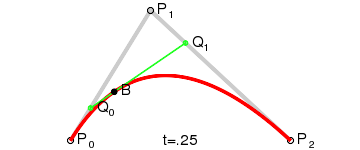
\includegraphics[height=2cm]{./figs/Bezier_2_big} & \parbox{5cm}{points $Q_0$ and $Q_1$ vary linearly from $P_0\rightarrow P_1$ and $P_1\rightarrow P_2$}\\
  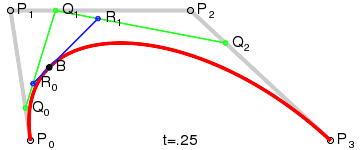
\includegraphics[height=2cm]{./figs/Bezier_3_big} & \parbox{5cm}{$Q's$ vary linearly, $R's$ vary quadratically}\\
  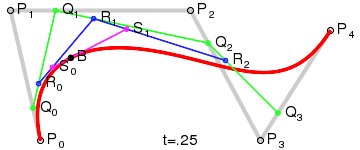
\includegraphics[height=2cm]{./figs/Bezier_4_big} & \parbox{5cm}{all within the hull of the control points }\\
  \end{tabular}
\end{frame}
%%%%%%%%%%%%%%%%%%%%%%%%%%%%%%%%%%%%%%%%%%%%%%%%%%%%%%%%%%%%%%%%%%%%%%%%
\begin{frame}
\frametitle{Bernstein Polynomial}
The $nth$-degree Bezier Polynomial through the $n+1$ points is given by
\begin{equation*}
  p(t) = \sum_{i=0}^{n}\begin{pmatrix}n\\i\\\end{pmatrix}(1-t)^{n-i}t^{i} p_i
\end{equation*}
where
\begin{equation*}
  \begin{pmatrix}n\\i\\\end{pmatrix} = \frac{n!}{i!(n-i)!}
\end{equation*}
For $n=3$ (cubic) we have
\begin{align*}
  x(t) & = (1-t)^3 x_0 + 3(1-t)^2 t x_1 + 3(1-t)t^2 x_2 + t^3 x_3\\
  y(t) & = (1-t)^3 y_0 + 3(1-t)^2 t y_1 + 3(1-t)t^2 y_2 + t^3 y_3
\end{align*}
\begin{block}{}
  plot\_bernstien.m
\end{block}
\end{frame}
%%%%%%%%%%%%%%%%%%%%%%%%%%%%%%%%%%%%%%%%%%%%%%%%%%%%%%%%%%%%%%%%%%%%%%%%
%%%%%%%%%%%%%%%%%%%%%%%%%%%%%%%%%%%%%%%%%%%%%%%%%%%%%%%%%%%%%%%%%%%%%%%%
\begin{frame}
\frametitle{Cubic Bezier Curve}
\begin{align*}
  x(t) & = (1-t)^3 x_0 + 3(1-t)^2 t x_1 + 3(1-t)t^2 x_2 + t^3 x_3\\
  y(t) & = (1-t)^3 y_0 + 3(1-t)^2 t y_1 + 3(1-t)t^2 y_2 + t^3 y_3
\end{align*}
Notice that $(x(0),y(0))=p_0$ and $(x(1),y(1))=p_3$.  So the Bezier
curve interpolates the endpoints but not the interior points.
\bigskip

\begin{center}
  \pgfimage[width=7cm]{./figs/bezier1}
\end{center}

\end{frame}
%%%%%%%%%%%%%%%%%%%%%%%%%%%%%%%%%%%%%%%%%%%%%%%%%%%%%%%%%%%%%%%%%%%%%%%%
%%%%%%%%%%%%%%%%%%%%%%%%%%%%%%%%%%%%%%%%%%%%%%%%%%%%%%%%%%%%%%%%%%%%%%%%
\begin{frame}
\frametitle{Bezier Curves}
\begin{align*}
  x(t) & = (1-t)^3 x_0 + 3(1-t)^2 t x_1 + 3(1-t)t^2 x_2 + t^3 x_3\\
  y(t) & = (1-t)^3 y_0 + 3(1-t)^2 t y_1 + 3(1-t)t^2 y_2 + t^3 y_3
\end{align*}
Notice:
\begin{enumerate}
  \item $P(0)=p_0$ and $P(1)=p_3$
  \item The slope of the curve at $t=0$ is a secant:
\begin{equation*}
  \frac{dy}{dx} = \frac{dy}{dt}\frac{dt}{dx} = \frac{3(y_1-y_0)}{3(x_1-x_0)}
  = \frac{y_1-y_0}{x_1-x_0}
\end{equation*}
  \item The slope of the curve at $t=1$ is a secant between the last two
control points.
  \item The curve is contained in the convex hull of the control points
\end{enumerate}
\end{frame}
%%%%%%%%%%%%%%%%%%%%%%%%%%%%%%%%%%%%%%%%%%%%%%%%%%%%%%%%%%%%%%%%%%%%%%%%
%%%%%%%%%%%%%%%%%%%%%%%%%%%%%%%%%%%%%%%%%%%%%%%%%%%%%%%%%%%%%%%%%%%%%%%%
\begin{frame}
\frametitle{Bezier Curves}
\begin{align*}
  x(t) & = (1-t)^3 x_0 + 3(1-t)^2 t x_1 + 3(1-t)t^2 x_2 + t^3 x_3\\
  y(t) & = (1-t)^3 y_0 + 3(1-t)^2 t y_1 + 3(1-t)t^2 y_2 + t^3 y_3
\end{align*}
Easier construction given points $p_0, \dots,p_3$:
\begin{align*}
  P(t) & = \begin{bmatrix}t^3&t^2&t^1&t^0\end{bmatrix}
           \begin{bmatrix}
           -1 &  3 & -3 & 1\\
            3 & -6 &  3 & 0\\
           -3 &  3 &  0 & 0\\
            1 &  0 &  0 & 0\\
           \end{bmatrix}
            \begin{bmatrix}p_0\\p_1\\p_2\\p_3\\\end{bmatrix}
\end{align*}
\begin{block}{}
see \texttt{bezier\_demo.m} from Mathworks File Exchange

\url{http://www.math.psu.edu/dlittle/java/parametricequations/beziercurves/index.html}
\end{block}
\end{frame}
\begin{frame}{Vector Graphics, Fonts, Adobe}
  Vector Graphics include primitives like
\begin{itemize}
  \item lines, polygons
  \item circles\
  \item { {\bf B\'ezier curves} }
  \item { {\bf B\'ezier splines} } or Bezigons
  \item text (letters created from {\bf B\'ezier} curves)
\end{itemize}

Flash Animation
\begin{itemize}
  \item Use {\bf B\'ezier curves} to construct animation path
\end{itemize}

Microsoft Paint, Gimp, etc
\begin{itemize}
  \item Use {\bf B\'ezier curves} to draw curves
  \item \url{http://msdn2.microsoft.com/en-us/library/ms534244.aspx}
\end{itemize}

Graphics
\begin{itemize}
  \item Use {\bf B\'ezier surfaces} to draw smooth objects
\end{itemize}
\end{frame}
\begin{frame}{B\'ezier Surfaces}
Take $(n,m)$.  That is, $(n+1,m+1)$ control points $p_{i,j}$ in 2d.  Then let
\begin{equation*}
  \vP(t,s) = \sum_{i=0}^{n} \sum_{j=0}^m \phi_{ni}(t) \phi_{mj}(s) \vp_{ij}
\end{equation*}
Where, again, $\phi_{ni}$ are the Bernstein polynomials:
\begin{equation*}
  \phi_{ni}(t) = \begin{pmatrix}n\\i\end{pmatrix} (1-t)^{n-i} t^i
\end{equation*}
  \begin{itemize}
  \item again, all within the convex hull of control points
  \item \url{http://www.math.psu.edu/dlittle/java/parametricequations/beziersurfaces/index.html}
  \end{itemize}
\end{frame}
\end{document}
